\documentclass{sig-alternate}


\usepackage{graphicx}

\newcounter{theorems}
\newtheorem{theorem}[theorems]{Theorem}

\begin{document}


\title{Probablistic Association Discovery using Functions of
  Observation Graph} 
\numberofauthors{2}

\author{
  \alignauthor 
  Hesen Peng \\
  \affaddr{Independent}\\
  \affaddr{136 102nd Ave SE Apt 326}\\
  \affaddr{Bellevue, Washington, USA 98004}\\
  \email{hesen.peng@gmail.com}  
  \alignauthor
  Tianwei Yu\\
  \affaddr{Dept of Biostatistics and Bioinformatics}\\
  \affaddr{Emory University}\\
  \affaddr{1518 Clifton Rd NE 3F}\\
  \affaddr{Atlanta Georgia, USA 30322}\\
  \email{tianwei.yu@emory.edu}
}

\date{\today{}}

\maketitle
 

\begin{abstract}
  Probablistic association discovery aims to identify the association
  between random vectors of their association, regardless of number of
  variables involved or linear/nonlinear functional forms. Application
  to high-dimensional data analysis has generated rising interest in
  probablistic association discovery.

  We developed a framework for probablistic association discovery on
  the Euclidean space using functions on the observation graph. We
  first discuss the property of mean observation distance and its
  novel application to association discovery. Then we generalize the
  advantageous property to a group of functions on the observation
  graph. The group of functions encapsulates major existing methods in
  association discovery, like mutual information and Mira score. We
  conducted numerical comparison that shows differentiated testing
  power under multiple scenarios. 

\end{abstract}


\category{H.4}{Information Systems Applications}{Miscellaneous}
\category{D.2.8}{Software Engineering}{Metrics}[complexity measures, performance measures]

\terms{Theory, Happy}

\keywords{ACM proceedings, \LaTeX, text tagging}


\section{Introduction}
\label{sec:intro}

In this paper we would like to propose and generalize new methods to
discover probablistic association between random vectors. Consider two
random vectors $X$ and $Y$ and $n$ pairs of independent and
indentically distributed (i.i.d.) random samples $\{X_i,
Y_i\}_{i=1}^n$. We would like to draw inference for the existence of
probablistic association between $X$ and $Y$ based on the $n$ pairs of
samples. The discussion in this paper will focus on the probablistic
association between continuous random variables defined in the
Euclidean space. However, general theory developed in this paper can
be applied in other spaces as well.

Classical association statistics like Pearson's correlation
coefficient assume functional forms (for example, piecewise linear,
monotonicity) between $X$ and $Y$, which are judged as
\emph{correlated} if
\begin{displaymath}
  Corr(X,Y) \ne 0
\end{displaymath}
Probablistic association statistic, as the name suggests, perceives
associations from the level of probablistic dependence. That is, $X$
and $Y$ are judged as independent if and only if their joint
probability density function can be factored
\begin{equation}
  \label{eq:independence}
  F(X,Y)= F(X) F(Y)
\end{equation}
where $F(\cdot)$ is the probability density function for the random
vector under consideration. Probabblistic association encapsulates a
larger group of associations than traditional correlation coefficient.
For example, probablistic association would consider nonlinear
interactions involving multiple variables.

We have noticed multiple of methods on probablistic association
discovery linked to functions on the observation distance graph. The
distance graph consists of nodes representing each observation $(X_i,
Y_i)$ in the $p+q$ Euclidean space. Here $p$ and $q$ are the
dimensions of $X$ and $Y$, respectively. Edges of the observation
graph would connect two nodes (observations) if specific criteria is
satisfied.

For example, mutual information and its derivatives have been the most
popular probablistic association statistic to
date\cite{cite:my-cas-work, citation:MINE-science,
  tostevin2009mutual}. To estimate mutual information, the joint
entropy can be approximated using $K$-nearest neighbour distance
averaged for each observation \cite{PhysRevE.69.066138, leonenko2008,
  doi:10.1080/104852504200026815}.

Recent breakthrough on distance covariate \cite{székely2009,
  székely2007} sheds light on universal association discovery with
its simplicity of form and theoretical flexibility. Brownian distance
\cite{székely2009} covariate proposed \texttt{dCov} as
\begin{equation*}
  V_N^2 = \frac{1}{n^2}\sum_{k,l=1}^n D^{X}_{kl}D^{Y}_{kl}
\end{equation*}
where $D^{X}_{kl}$ and $D^{Y}_{kl}$ are simple linear functions of
pairwise distances between sample elements calculated on $X$ and $Y$
dimensions, respectively. Given fixed marginal distribution for $X$
and $Y$, large Brownian distance covariate suggests the existence
of probablistic association. 

In an independent research, the authors proposed Mira score
\cite{my-dissertation} as
\begin{equation*}
  M = \sum_{k,l = 1}^n D^{(X,Y)}_{kl} w_{kl}
\end{equation*}
where $D^{(X,Y)}_{kl}$ is the distance between sample elements
calculated using both $X$ and $Y$ dimensions, and $w_{kl}=1$ when the
involved elements are nearest neighbors, $w_{kl}=0$ otherwise. Given
fixed marginal distribution for $X$ and $Y$, small Mira score suggests
the existence of probablistic association. 

We would like to discuss the property of functions applied to the
distances of the observation graph. The discussion of the section
below is inspired by comparing mean observation distance between
dependent and independent random vectors of the same marginal
distribution. Our intution suggest that when two random vectors are
probablistically associated, their observation distances tend to be
smaller than their independent counterparts.

Take Figure \ref{fig:comparison} for example, both plots show 300
samples from two bivariate random vectors. Observations on the left
panel are sampled from independent bivariate normal distributions.
Observations on the right panel are sampled from mixture bivariate
normal distribution with $\pm 0.8$ covariates. Coincidentally, both
distributions have standard normal mariginal distribution and zero
coerrelation coefficient. However, the two samples differ on a group
of metrics defined on the observation distances. Table
\ref{tab:example-compare} shows the mean distance, mean nearest
neighbour distance, and mean log-nearest neighbour distance are all
smaller for the dependent case compared with independent case. We have
repeated the simulation multiple times and the same trend is observed
in large probability.

\begin{figure}[t]
  \centering
  \includegraphics[width=.5\textwidth,height=.25\textwidth]{../code/visualize/plot/example-1.eps}
  \caption{Random samples generated from independent bivariate normal
    distribution (left), and mixture bivariate normal distribution
    with $\pm 0.8$ covariates (right). The dashed lines connects two
    observations if they are nearest neighbours.}
  \label{fig:comparison}
\end{figure}

% latex table generated in R 3.0.2 by xtable 1.7-3 package
% Fri Aug  1 16:43:52 2014
\begin{table}[ht]
  \centering
  \begin{tabular}{lrr}
    \hline
    Metric & Left (Ind) & Right (Mix. Normal) \\ 
    \hline
    mean distance & 1.81 & 1.70 \\ 
    mean NN & 0.14 & 0.12 \\ 
    mean $\log(\textrm{NN})$ & -2.24 & -2.43 \\ 
    \hline
  \end{tabular}
  \caption{Comparison between the independent bivariate normal
    distribution and mixture normal distribution in Figure
    \ref{fig:comparison}.  Statistics used in the comparison include
    mean observation distance, mean nearest neighbour distance, mean
    log-nearest neighbour distance. }
  \label{tab:example-compare}
\end{table}

The above observation is no coincidence. In this article we will
generalize the functions on the observation graph, discuss their
properties in identifying probablistic associations. More
specifically, we will contribute:
\begin{enumerate}
\item Point out that non-trial monotonic functions of the observation
  graph would be capable of discoverying universal association.
\item Present numerical comparison between existing methods.
\end{enumerate}
For illustration purpose we applied the proposed methods to the
association identication in image analysis and text mining. The
results are very interesting.

\section{Theory}
\label{sec:funcs}

% Given $n$ pairs of random samples $\{X_{i},Y_{i}\}_{i=1}^n$, we are
% interested in inferring the existence of probablistic association
% between these two random vectors. Denote the observation distance as
% $D=(d_{ij})_{n\times n}$, where $d_{ij}$ is the Euclidean distance
% between the $i$ and $j$-th observation calculated using both $X$ and
% $Y$ dimensions. That is
% \begin{displaymath}
%   d_{ij} = \sqrt{\sum_{l = 1}^p (X_{il} - X_{jl})^2 + \sum_{k = 1}^q (Y_{ik} - Y_{jk})^2}
% \end{displaymath}
% In the mean time, consider a parallel pair of random vectors $(\hat{X},
% \hat{Y})$, where $\hat{X}$ and $\hat{Y}$ share the identical marginal distribution
% as $X$ and $Y$, respectively. The only difference is that the random
% vectors $\hat{X}$ and $\hat{Y}$ are independent of each other. When we take
% $n$ pairs of independent samples from $(\hat{X}, \hat{Y})$ 

We are interested in testing the existence of probablistic association
between two random vectors $(X,Y)$, given $n$ pairs of observations.
Consider another pair of random vectors $(\hat{X}, \hat{Y})$, where
$\hat{X}$ follows independent and identical distribution
(\emph{i.i.d.}) as $X$ and $\hat{Y}$ follows \emph{i.i.d.} as $Y$. The
only difference is that $\hat{X}$ and $\hat{Y}$ are mutually
independent. As mentioned above, we would like to compare the sample
observation distance from $(X,Y)$ against that from
$(\hat{X},\hat{Y})$.
\begin{thm}
  \label{thm:1}
  Denote the distance between two independent random samples from
  $(X,Y)$ as $d_{XY}$, and the distance between two independent random
  samples from $(\hat{X},\hat{Y})$ as $d_{\hat{X}\hat{Y}}$. Then we
  have
  \begin{displaymath}
    E(d_{XY}) \le E(d_{\hat{X}\hat{Y}})
  \end{displaymath}
\end{thm}
For the sake of space, proofs of the theoretical results in this
section are presented in Appendix \ref{sec:proof}. Theorem \ref{thm:1}
above confirms our earlier intuition: when two random vectors are
probablistically associated, their observations tend to be closer
compared with their independent counterparts. 




%% here talk about asymptotic property (normality). 

%% here talk about the functions of these values using delta methods. 

%% here talk about the nearest neighbour property. 

\section{Numerical comparison}
\label{sec:comparison}

\section{Applications}
\label{sec:haha}



\appendix{}

\section{Proof of Theorems}
\label{sec:proof}

\begin{proof}[Theorem \ref{thm:1}]
  We would like to make the following definitions before proceeding:
  \begin{itemize}
  \item $(X', Y')$: follows \emph{i.i.d.} as $(X,Y)$
  \item $(\hat{X},\hat{Y})$: $\hat{X}$ follows \iid{} as $X$;
    $\hat{Y}$ follows \iid{} as $Y$. But $\hat{X}$ and $\hat{Y}$ are
    independent. $(\hat{X},\hat{Y})$ is independent of all previously
    defined random variables.
  \item $(\hat{X}', \hat{Y}')$: follows \emph{i.i.d.} as
    $(\hat{X},\hat{Y})$ and is independent of all the above random
    variables.
  \end{itemize}
  Based on the abvoe definition, the distance between independent
  random pairs of observations from $(X,Y)$ and its independent
  counterpart $(\hat{X}, \hat{Y})$ can be expressed as: 
  \begin{eqnarray*}
    E(d_{XY}) & = & E(|(X,Y) - (X', Y')|_{p+q})\\
    E(d_{\hat{X}\hat{Y}}) & = & E(|(\hat{X},\hat{Y}) - (\hat{X}', \hat{Y}')|_{p+q})\\
  \end{eqnarray*}
  Further more, based on Equation 2.5 of \cite{székely2007}, we have:
  \begin{eqnarray*}
    E(|(X,Y) - (X',Y')|_{p+q}) &=& \int_{R^{p+q}}
    \frac{1-|f_{X,Y}(s,t)|^2}{C_{p+q}|(t,s)|_{p+q}^{1+p+q}} d(s,t)\\
    E(|(\hat{X},\hat{Y}) - (\hat{X}',\hat{Y}')|_{p+q}) &=& \int_{R^{p+q}}
    \frac{1-|f_{\hat{X},\hat{Y}}(s,t)|^2}{C_{p+q}|(t,s)|_{p+q}^{1+p+q}} d(s,t)\\
  \end{eqnarray*}
  where $f_{X,Y}(s,t)$ is the characteristics functions of $(X,Y)$;
  $f_{\hat{X},\hat{Y}}(s,t)$ is the characteristics functions of
  $(\hat{X},\hat{Y})$; $C_{p+q}$ is a constant defined in Equation 2.3
  of \cite{székely2007}.

  Meanwhile, the characteristics function of $(\hat{X}, \hat{Y})$ can
  be factored because of their independence
  \begin{displaymath}
    f_{\hat{X},\hat{Y}}(s,t) = f_{\hat{X}}(s) f_{\hat{Y}}(t) 
  \end{displaymath}
  Summarizing the above, we have 
  \begin{eqnarray*}
    E(d_{XY} - d_{\hat{X}\hat{Y}})& =& \int_{R^{p+q}} \frac{|f_X(s)
      f_Y(t)|^2 - |f_{XY}(s,t)|^2}{C_{p+q}|(t,s)|_{p+q}^{1+p+q}}
    d(t,s)\\
    &\ge & 0 
  \end{eqnarray*}
  according to Cauchy-Schwarz inequality. 
\end{proof}


\bibliographystyle{abbrv}
\bibliography{mira-score}


\end{document}
